%! TEX root = ../../master.tex
\lecture[Matroids. Greedy works only on matroids.]{Di 17 May 2022}{Matroids}
\begin{definition}[Greedy]
    Given a set $\mathcal{I} \subset \mathcal{P}(E)$. We call following class of algorithms
    $\vocab{greedy}$:
    \\
    \begin{algorithm}[H]
        \SetAlgoLined
        sort $w_1 \geq \dots \geq w_m$\\
        $T \leftarrow \emptyset$\\
        \For{$i=1,...,m$}{
            \If{$T \cup e_i \in \mathcal{I}$}{
                $T \leftarrow T \cup e_i$\\
            }
        }
        \caption{General greedy algorithm}
    \end{algorithm} \noindent
\end{definition}
\begin{theorem}
    The $\LP$s \eqref{eq:kruskal_alt} and \eqref{eq:kruskal_dual}
    can be solved greedily with \emph{any} submodular function $r$.
\end{theorem}
\begin{proof}
    We show that it suffices to choose for $i=1,\dots,m$ greedily $x_{e_i}$ as big as possible, i.e.
    \begin{align*}
        x_{e_1} & \coloneqq r(S_1)        \\
        x_{e_2} & \coloneqq r(S_2)-r(S_1) \\
                & \vdots
    \end{align*}
    It is clear that $x \geq 0$. Thus, consider $S \subseteq E$ in order to show $x(S) \leq r(S)$.
    Let $k \coloneqq \max \{i \mid e_i \in S\}$. Using induction over $k$ with the trivial base case $k=0$,
    we define $S' \coloneqq S \setminus e_k$. Observe, by choice of $k$, that
    $S \cap S_{k-1} = S'$ and $S \cup S_{k-1} = S_k$.
    Therefore, by submodularity \ref{thm:submodularity}:
    \begin{align*}
        r(S) \geq r(S') + r(S_k) - r(S_{k-1})
    \end{align*}
    Induction on $k$ yields $x(S') \leq r(S')$, and thus
    \begin{align*}
        x(S) & = x(S') + x_{e_k}=x(S')+r(S_k)-r(S_{k-1}) \\
             & \leq r(S')+ r(S_k) - r(S_{k-1})           \\
             & \leq r(S)
    \end{align*}
\end{proof}
\begin{note}
    Assuming non-degeneracy, then the vertices of the submodular polyhedron
    correspond to permutations of $E$. In particular, there are $m!$ vertices.
\end{note}
% Consider permutation. Then $y^*_S$ is dual feasible,  and $y_{S_i}^*=w_i - w_{i-1}$, and $y^*_{S_i} \geq 0$.
% Now, $\sum_{S:e\in S} y_S^* \geq w_e$.
% This shows for all $e \in E$: $\sum_{S: e \in S} y_S^* = w_e$.
Now, let's concentrate on submodular functions where $r(\{e_i\}) \in \{0,1\}$.
We can derive this notion with matroids - a common generalisation of (combinatorial) graphs/matrices that
define "independence".
\begin{definition}[Matroid]
    Given a set $\mathcal{I} \subset \mathcal{P}(E)$. If also
    \begin{enumerate}
        \item $\emptyset \in \mathcal{I}$,
        \item $S \in \mathcal{I}, R \subset S \Rightarrow R \in \mathcal{I}$, and
        \item $R,S \in \mathcal{I}, |R|< |S| \Rightarrow \exists e \in S\setminus R: R+e\in \mathcal{I}$,
    \end{enumerate}
    then $\mathcal{I}$ is a \vocab{matroid}. If only properties (1) and (2) hold, we call it a \vocab{independence system}.
    Property (3) is also called \vocab{extensibility}.
\end{definition}
\begin{definition}[Rank function]
    Given a matroid $\mathcal I$. Define the \vocab{rank function} $r : \mathcal P(E) \rightarrow \integers$ as
    \begin{align*}
        r(S) = \max_{I \in \mathcal{I}, I \subset S} |I|.
    \end{align*}
\end{definition}
\begin{theorem}
    For all matroids, the rank function is submodular.
\end{theorem}
\begin{proof}
    It suffices to show for $R \subsetneq S \subsetneq S+e$ that
    \begin{align*}
        \underbrace{r(S+e) - r(S)}_{0,1} \leq \underbrace{r(R+e) - r(R)}_{0,1}.
    \end{align*}
    The only bad case is $r(S+e)-r(S)=1$ and $r(R+e)-r(R)=0$.
    Suppose
    \begin{align*}
        r(R) & = |I_1|, I_1 \in \mathcal{I}, I_1 \subset R \\
        r(S) & = |I_2|, I_2 \in \mathcal{I}, I_2 \subset S
    \end{align*}
    Set $k = r(S)-r(R) \geq 0$.
    From $R \subsetneq S$ and extensibility follows that
    there is a $K \subset S \setminus R$ with $|K|=k$ such that
    \begin{align*}
        I_2=I_1 \cup K
    \end{align*}
    Also, from $r(S+e) > r(S)$ it follows from extensibility, that there is $f \in S + e$ such that $I_2+f \in \mathcal{I}$.
    We see that $f=e$, otherwise it follows from $I_2+f \subset S$ that $r(S) > |I_2|$, which is a contradiction.

    Summarizing, we see $I_2+e \in \mathcal{I}$.
    From property (2) follows that $I_1+e \in \mathcal{I}$.
    Also $I_1 +e \subset R +e$, which implies $r(R+e)=r(R)+1=|I_1|+1$. This contradicts our initial assumption!
\end{proof}
\begin{corollary}
    Greedy is optimal for \emph{any} matroid.
\end{corollary}
\begin{theorem} \label{thm:greedy-ind-is-matroid}
    If Greedy is optimal for all cost vectors $w$ on an independence system, then it is a matroid.
\end{theorem}
Let $(E,\mathcal{I})$ be an independence system. Then extensibility states
that additionally all maximal independent subsets of $S$ have the same size, and are thus $\emph{maximum}$.
\begin{example}
    Note the difference of \emph{maximal} and \emph{maximum}! Given following graph:
    \\
    \begin{minipage}{\textwidth}
        \centering
        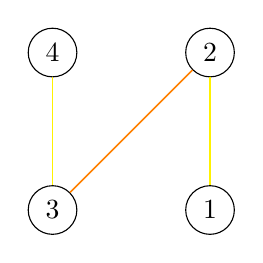
\begin{tikzpicture}
            \begin{scope}[
                    every node/.style={circle, draw},
                    every edge/.style={draw, semithick}
                ]

                \node (1) at (2,0) {$1$};
                \node (2) at (2,2) {$2$};
                \node (3) at (0,0) {$3$};
                \node (4) at (0,2) {$4$};

                \path[draw=orange] (2) edge (3);
                \path[draw=yellow] (1) edge (2);
                \path[draw=yellow] (3) edge (4);
            \end{scope}
        \end{tikzpicture}
        % \captionof{figure}{A graph with the spanning tree in black and arc subset $S$ in orange}
    \end{minipage}
    Then the yellow edges form only a maximal matching, while the orange edges a maximum (and maximal) matching.
\end{example}
Define
\begin{align*}
    \rho(S) = \min \{|I|\mid I \subset S, I \in \mathcal{I}, I\ \text{maximal}\}.
\end{align*}
Especially, for matroids $\rho(S)=r(S)$.

We want to prove a stronger theorem, though:
\begin{theorem} \label{thm:greedy-bad}
    If we apply Greedy to an independence system $(E, \mathcal{I})$, then it holds
    \begin{align*}
        q \coloneqq \min_{S \subset E} \frac{\rho(S)}{r(S)}\leq \frac{\text{greedy obj. value}}{\text{optimal obj. value}} \leq 1
    \end{align*}
    Additionally, the worst case is attainable.
\end{theorem}
\begin{proof}
    Consider $w_{e_1} \geq ... \geq w_{e_n}$ and $S_i\coloneqq\{e_1,...,e_i\}$.
    Let $G \subset E$ be a greedy solution and $G_k \coloneqq G \cap S_k$.
    Let $O \subset E$ be an optimal solution and $O_k \coloneqq G \cap O_k$.

    Consider two cases:
    \begin{itemize}
        \item $e_i \in G$: Then $|G_i| = |G_{i-1}| +1$
        \item $e_i \not \in G$: Then $|G_i|=|G_{i-1}|$
    \end{itemize}
    Therefore, the greedy objective value is
    \begin{align*}
        \sum_i (|G_i| - |G_{i-1}|)w_{e_i} & = \sum_i |G_i|(w_{e_i} - w_{e_{i+1}})         \\
                                          & \geq  \sum_i \rho(S_i)(w_{e_i} - w_{e_{i+1}}) \\
                                          & \geq q \sum_i r(S_i)(w_{e_i} - w_{e_{i+1}})   \\
                                          & \geq q \sum_i |O_i|(w_{e_i} - w_{e_{i+1}})    \\
                                          & = q \sum_i (|O_i|-|O_{i-1}|)w_{e_i}           \\
                                          & = q \cdot \ \text{optimal obj. value}
    \end{align*}

    Suppose our $q$ is attained at $S$,
    \begin{align*}
        q = \frac{\rho(S)}{r(S)}.
    \end{align*}
    By definition there are $I_1,I_2 \subset S$ with $I_1,I_2 \subset \mathcal{I}$
    such that $r(S)=|I_2|$ and $\rho(S)=|I_1|$.
    Choose
    \begin{align*}
        w_e = \begin{cases}
                  1, & e \in S      \\
                  0, & e \not \in S
              \end{cases}.
    \end{align*}
    and consider following ordering:
    \[
        \begin{NiceArray}{|c|c|c|}[last-row] \hline
            I_1 & S \setminus I_1 & S^c \\ \hline
                &                 &
            \CodeAfter
            \UnderBrace{1-1}{2-2}{w=1}
            \UnderBrace{1-3}{2-3}{w=0}
        \end{NiceArray}
    \]

    Greedy solution will be $I_1$ because of maximality, but optimal solution is $I_2$.
    Therefore $q = \frac{|I_1|}{|I_2|}$ as proposed.
\end{proof}
\begin{proof}[Proof for \autoref{thm:greedy-ind-is-matroid}]
    For matroids, $q=1$. Otherwise, $q < 1$.
\end{proof}
\begin{corollary}
    Greedy is a 2-approximation for matching.
\end{corollary}
\begin{example}
    Other matroids are given by:
    \begin{enumerate}
        \item Uniform: $\mathcal{I}=\{S \mid |S| \leq k\}$
        \item Partition: $E$ is partitioned into $P_1,...,P_k$. Then $I \in \mathcal{I}$ iff for all $i$, $|I \cap P_i| \leq 1$.
              \begin{enumerate}
                  \item  $G=(N,A),\ P_i = \delta^+(\{i\})$
                  \item  $G=(S \cup T,E),\ P_i=\delta(\{i\}), i \in S$
              \end{enumerate}
    \end{enumerate}
\end{example}
\begin{example}
    Independence systems, that are \emph{not} matroids, are for example:
    \begin{enumerate}
        \item Bipartite matching
        \item Branching: $G=(N,A)$, $B \subseteq A$ is a branching iff acyclic, i.e. for all $i$, $\delta^-(\{i\}) \leq 1$.
    \end{enumerate}
\end{example}
\begin{remark} \label{rmk:intersection_matroid}
    Intersections of matroids seem interesting:
    Previous examples can be generated via intersections of partition matroids,
    i.e. for a bipartite graph $G = (S \cup T, E)$, the set of bipartite matchings $M$ is given by
    \begin{align*}
        \mathcal I_1 & \coloneqq \{I \subset E \mid \forall i \in S: |I \cap \delta^+(\{i\})| \leq 1\} \\
        \mathcal I_2 & \coloneqq \{I \subset E \mid \forall i \in T: |I \cap \delta^+(\{i\})| \leq 1\} \\
        M            & = \mathcal I_1\cap \mathcal I_2.
    \end{align*}
    We can visualize this by coloring every partition set and defining the matroids as the subsets
    where we take at most one edge per color:
    \\
    \\
    \begin{minipage}{\textwidth}
        \centering
        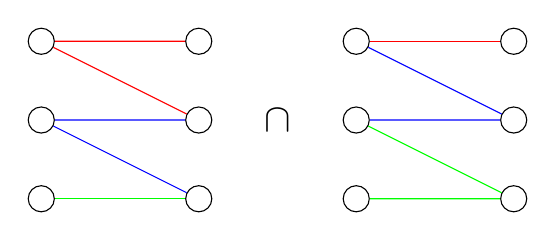
\begin{tikzpicture}
            \begin{scope}[
                    every node/.style={circle, draw},
                    every edge/.style={draw, semithick}
                ]

                \node (l1) at (0,0) {};
                \node (l2) at (0,1) {};
                \node (l3) at (0,2) {};
                \node (r1) at (2,0) {};
                \node (r2) at (2,1) {};
                \node (r3) at (2,2) {};

                \draw[green] (l1) -- (r1);
                \draw[blue] (r1) -- (l2) -- (r2);
                \draw[red] (r2) -- (l3) -- (r3);

                \node (l1) at (4,0) {};
                \node (l2) at (4,1) {};
                \node (l3) at (4,2) {};
                \node (r1) at (6,0) {};
                \node (r2) at (6,1) {};
                \node (r3) at (6,2) {};

                \draw[green] (l1) -- (r1) -- (l2);
                \draw[blue] (l2) -- (r2) -- (l3);
                \draw[red] (l3) -- (r3);
            \end{scope}
            \node (cap) at (3,1) {\Large$\cap$};
        \end{tikzpicture}
        % \captionof{figure}{A graph with the spanning tree in black and arc subset $S$ in orange}
    \end{minipage}
    \vspace{5pt}
    \\
    By taking the intersection we prohibit to take multiple edges from the same node, leaving us at bipartite matchings.
\end{remark}